\documentclass{beamer}
\usepackage[utf8]{inputenc}

\usetheme{Madrid}
\usecolortheme{default}

%used by me%
\usepackage{comment}
\usepackage{xcolor}

\usepackage{caption}
\usepackage{graphicx}
\usepackage{ragged2e}
\usepackage{subcaption}

\usepackage[style=apa,backend=bibtex]{biblatex}
\addbibresource{biblio.bib}

\usepackage{appendixnumberbeamer}
\newcommand{\backupbegin}{
   \newcounter{framenumbervorappendix}
   \setcounter{framenumbervorappendix}{\value{framenumber}}
}
\newcommand{\backupend}{
   \addtocounter{framenumbervorappendix}{-\value{framenumber}}
   \addtocounter{framenumber}{\value{framenumbervorappendix}} 
}


% Define custom color
\definecolor{darkskyblue}{RGB}{0, 103, 165}
\definecolor{darkgreen}{RGB}{0,128,0}
%used by me%

%\usepackage{enumitem}

%------------------------------------------------------------
%This block of code defines the information to appear in the
%Title page
\title[The ENACT proposal] %optional
{ENACT - ENergy efficiency through ArChitectural Tactics for Software Engineering}

%\subtitle{ENACT - ENergy efficiency through ArChitectural Tactics for Software Engineering}

\author[Tareq Chy] % (optional)
{Tareq Md Rabiul Hossain Chy\inst{1} \and Sophie Chabridon\inst{2} \and Denisse Munante\inst{3}}

\institute[]
{
	\inst{1}%
	École Des Mines de Saint-Étienne, Saint-Étienne \& SAMOVAR Lab, Évry, France
    \and
	\inst{2}%
	Télécom SudParis, Institut Polytechnique de Paris \& SAMOVAR Lab, Évry, France
	\and
	\inst{3}%
	ENSIIE \& SAMOVAR Lab, Évry, France
}
\date[August 30, 2023]
{Internship Defense, 30 August 2023}

\titlegraphic{
    \parbox[c]{1.7cm}{
\includegraphics[height=1.7cm]{figures/edm.png}}
     \parbox[c]{1.4cm}{
\includegraphics[height=1.3cm]{figures/logo_tsp.png}}
	 \parbox[c]{1cm}{
\includegraphics[width=.8cm,height=1.1cm]{figures/logo_ENSIIE.png}} 
	 \parbox[c]{1.9cm}{
\includegraphics[height=0.5cm]{figures/2022_logo_samovar.png}} \hspace{.45cm}
	 %\parbox[c]{2cm}{
\includegraphics[height=0.75cm]{figures/E4C_logo.png}} \hspace{.25cm}
	 
}

%End of title page configuration block
%------------------------------------------------------------

\begin{document}
\section{Main Content}
%---------- Slide 2(Outline) ------------%
\frame{\titlepage}
\begin{frame}{Main Content}
\frametitle{Outline}
\begin{itemize}
    \vspace*{-1.5cm} % Adjust the value to change the vertical position of the pictures
    \item Introduction
    \item Internship Objectives
    \item Research Contributions
    %\item Preliminary study for empirical evaluations
    \item Conclusion
    \item Next Steps
\end{itemize}
\end{frame}


%---------- Slide 3(Introduction) -----------%
\begin{frame}{Main Content}
\frametitle{Introduction: Importance of Energy Efficiency in Combating Global Warming}

\begin{figure}
    \vspace*{-0.8cm} % Adjust the value to change the vertical position of the pictures
    \centering
    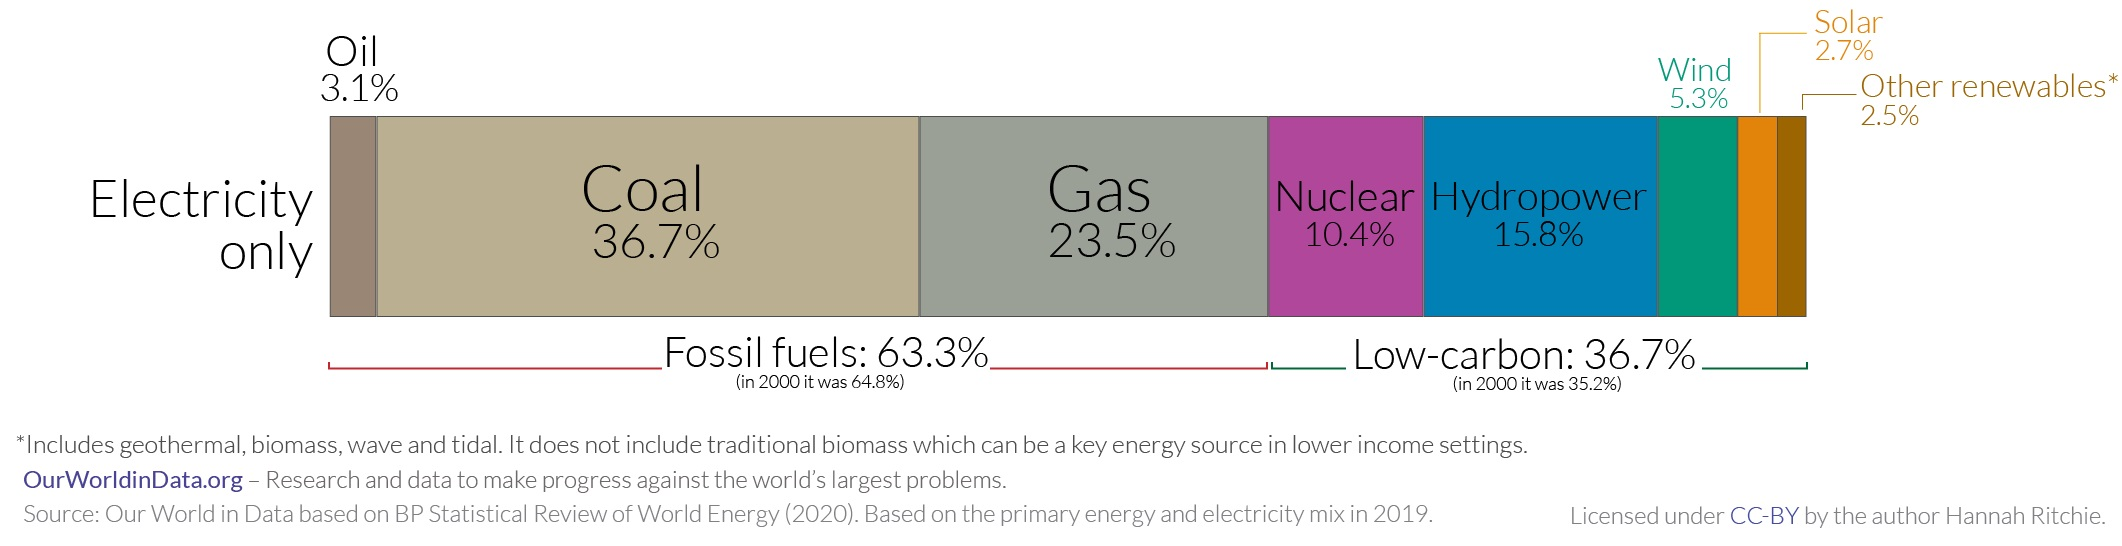
\includegraphics[width=1\textwidth]{figures/Global_electricity_from_fossil_fuels.jpg}
    \captionsetup{justification=centering, skip=0pt} % Center the caption and remove extra space
    \caption*{\scriptsize{\textcolor{blue}{Figure}: Global electricity production from fossil fuels \footnote{\tiny \url{https://ourworldindata.org/uploads/2020/08/Global-energy-vs.-electricity-breakdown-1536x812.png}}}}
    \label{fig:Global_electricity_from_fossil_fuels}
    
\end{figure}

 
\begin{itemize}
    \vspace*{-0.5cm} % Adjust the value to change the vertical position of the pictures
    \item \footnotesize Fossil fuels are the largest contributors to global climate change, accounting for 75\% of greenhouse gas emissions\footnote{\tiny \url{https://www.un.org/en/climatechange/science/causes-effects-climate-change}}.
    \item \footnotesize About 63.3\% of global electricity is produced from fossil fuels.
    \item \footnotesize Rising electricity consumption in various sectors: home, entertainment, IoT devices, etc.
\end{itemize}
\vspace*{-0.4cm}
\end{frame}

%---------- Slide 5(Internship objectives) -----------%
\begin{frame}{Main Content}
  \frametitle{Internship objectives}
  \vspace{-1cm}
  \textbf{\footnotesize Exploring tactics for software energy efficiency improvement.} 
  
  % Add an empty line here
  \vspace{1em}
  
  \footnotesize From this objective we define 2 research questions:
  \begin{itemize}
    \item \footnotesize \textbf{RQ1} Which tactics help to improve Energy Efficiency?
    \item \footnotesize \textbf{RQ2} How can we automatise the integration of tactics to reduce energy consumption?
        \vspace{1em}
        \begin{itemize}
            \item \footnotesize \textbf{RQ2.1} Does the improvement of \textit{execution time} and  \textit{memory consumption} reduce energy consumption?
            \item \footnotesize \textbf{RQ2.2} Could code refactoring integrate into GI? Which elements need to be extended in the Gin tool?
            \item \footnotesize \textbf{RQ2.3} In which extent code refactoring genetically improve the software to reduce energy consumption?
      \end{itemize}
  \end{itemize}
\end{frame}

%---------- Slide 6(Research Contributions:) -----------%
\begin{frame}{Main Content}
  \frametitle{Research Contributions:}
  \textbf{\footnotesize RQ1: Which tactics help to improve Energy Efficiency?}
  
  \begin{figure}
    \centering
    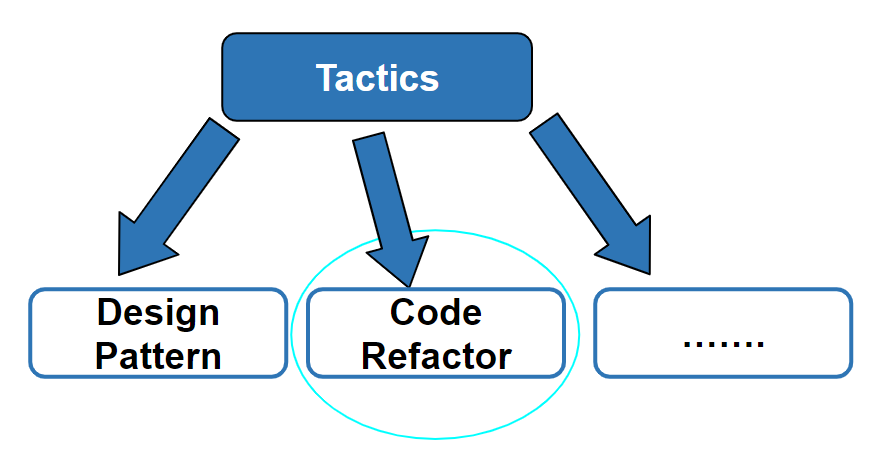
\includegraphics[width=.6\textwidth]{figures/Slide_12(Tactics to improve energy efficiency).png}
 \end{figure}
 
 \begin{figure}
    \centering
    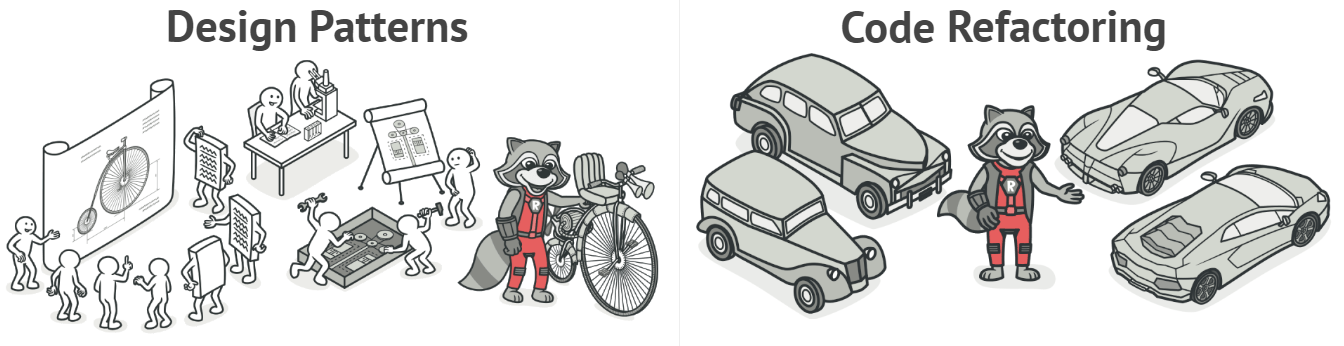
\includegraphics[width=1\textwidth]{figures/Slide_12(Code refactoring and design pattern).png}
 \end{figure}
  
\end{frame}
%---------- Slide 7(Research Contributions) -----------%
\begin{frame}{Main Content}
  \frametitle{Research Contributions(RQ1): Code refactoring techniques}

\small {\footnotesize Code refactoring can improve code efficiency and energy consumption, but its impact varies based on the specific techniques used.}
\hypertarget{back}{}
  \begin{itemize}
     \item \textbf{\footnotesize Positive Impact in Energy Efficiency:}
     \begin{itemize}
        \item \footnotesize Convert Local Variable to Field
        \item \footnotesize Introduce Parameter Object
        \item \footnotesize Inline Temp
        \item \footnotesize Move Method
        \item \footnotesize Simplify Nested Loop
        \item \footnotesize Encapsulate Field
    \end{itemize}
    
    \item \textbf{\footnotesize Context-Dependent Impact in Energy Efficiency:}
     \begin{itemize}
        \item \footnotesize Extract Local Variable
        \item \footnotesize Extract Method
        \item \footnotesize \hyperlink{codeRefactorSlide}{Inline Method}
        \item \footnotesize Introduce Indirection
    \end{itemize}

  \end{itemize}

\end{frame}


%---------- Slide 8(Research Contributions)  -----------%
\begin{frame}{Main Content}
  \frametitle{Research Contributions: Genetic Improvement toward Energy Efficiency}

  \vspace*{-.2cm} % Adjust the value to change the vertical position of the text
  
  \textbf{\footnotesize RQ2: How  can we automatise the integration of tactics to reduce energy consumption?}
 \vspace*{-.5cm} % Adjust the value to change the vertical position of the text
  \begin{figure}
    \centering
    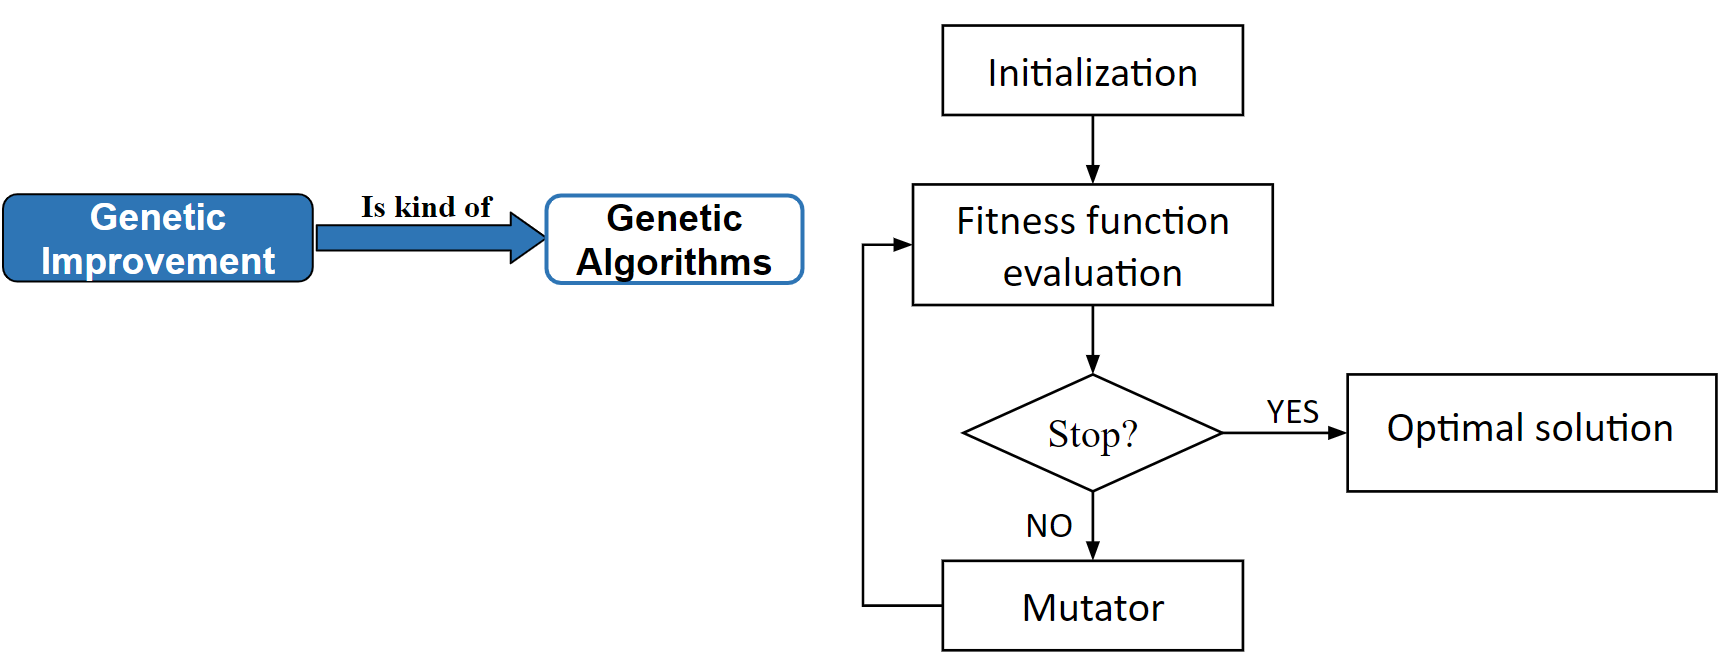
\includegraphics[width=.7\textwidth]{figures/Slide_14(Genetic Improvement).png}
    \caption*{\scriptsize{\textcolor{blue}{Figure}: Overall process of genetic improvement}}
 \end{figure}
 
 \vspace{-.8em}
\footnotesize{\cite{DBLP:conf/gecco/ZuoBP22} examined the usability of Genetic Improvement (GI) tools. Only 2 tools, Gin\footnote{\tiny \url{https://github.com/gintool/gin}} and PyGGI\footnote{\tiny \url{https://github.com/coinse/pyggi}}, could be readily applied for software improvement.}
\vspace{.5em}

\footnotesize{\footnotesize Gin is specifically designed for the Java ecosystem. Selected for research due to Java's lower energy consumption compared to Python.}
 
 
\end{frame}



%---------- Slide 9(Research Contributions) -----------%
\begin{frame}{Main Content}
  \frametitle{Research Contributions(RQ2): The Gin toolbox }
  \vspace*{-.5cm} % Adjust the value to change the vertical position of the text
  \begin{itemize}
    \item \footnotesize Gin is an experimental substrate for Genetic Improvement (GI), a field of software engineering research that aims to improve existing software through search-based techniques. 
  \end{itemize}
  
  \begin{figure}
    \centering
    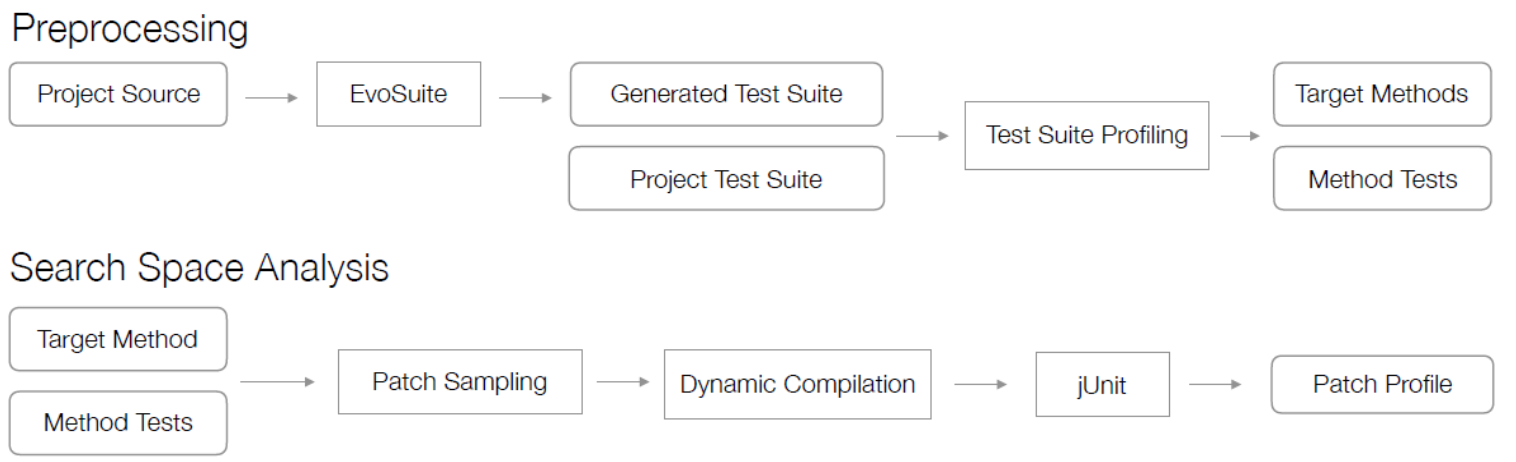
\includegraphics[width=1\textwidth]{figures/Slide_16(Gin pipelines).png}
    \caption*{\scriptsize{\textcolor{blue}{Figure}: Gin pipelines from \cite{brownlee2019gin}}}
  \end{figure}
 
\end{frame}


%---------- Slide 10(Research Contributions)  -----------%
\begin{frame}{Main Content}
  \frametitle{Research Contributions(RQ2.1): Does the improvement of execution time and memory consumption reduce energy consumption?}
  \vspace{-.2cm}
  \begin{table}
    \centering
    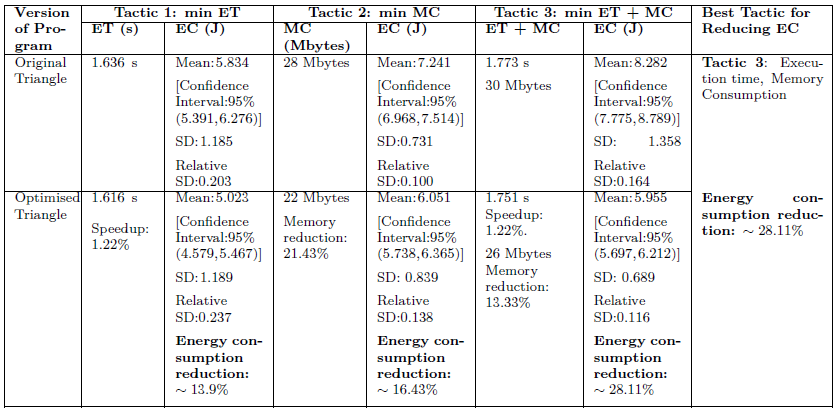
\includegraphics[width=\textwidth]{figures/Result_table_f.png}
    \caption*{\tiny{\textcolor{blue}{Table}: Comparison of the energy consumed by the original vs. the optimized versions of the studied programs, \textit{where: ET=execution time in seconds, MC=memory consumption in Megabytes, EC=energy consumption in Joules}}}
  \end{table}
\end{frame}

%---------- Slide 11(Research Contributions Triangle)  -----------%
\begin{frame}{Main Content}
  \frametitle{Research Contributions(RQ2.1): Does the improvement of execution time and memory consumption reduce energy consumption?}

  \begin{figure}
    \centering
    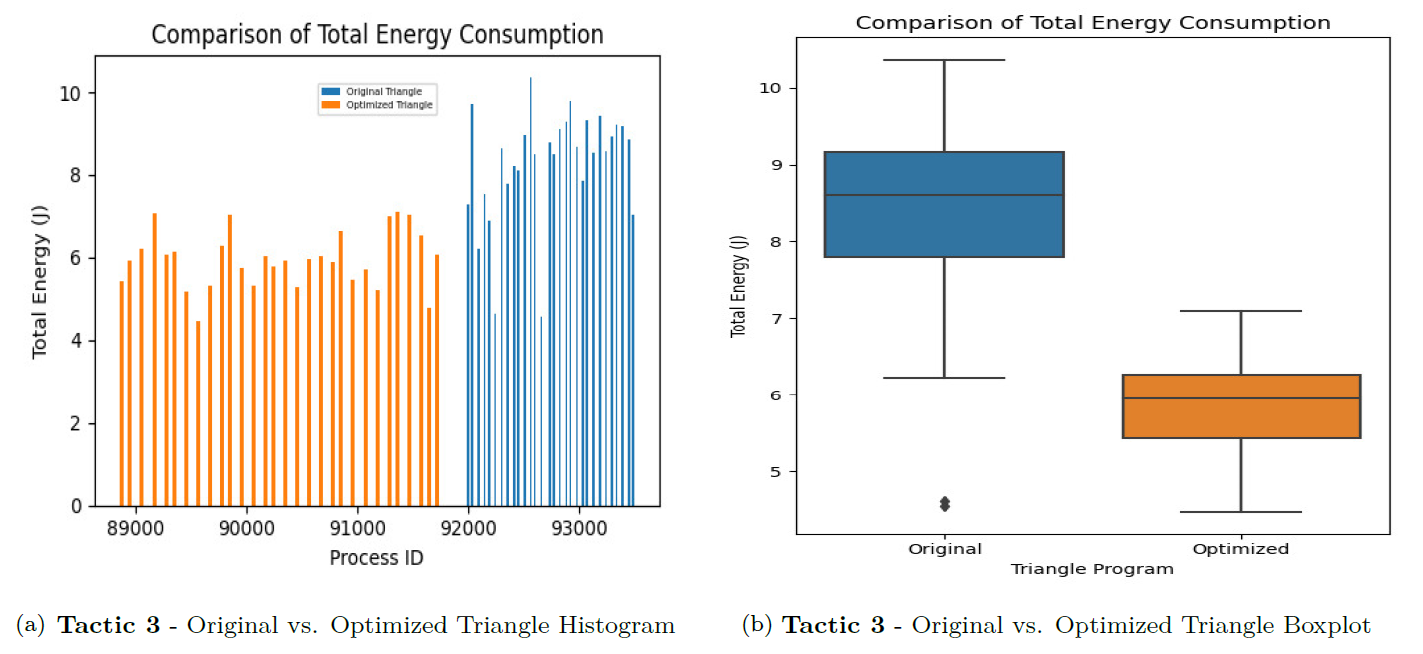
\includegraphics[width=1\textwidth]{figures/Hiegest_Triangle.png}
    \caption*{\scriptsize{\textcolor{blue}{Figure}: Energy consumption comparison for the original vs. optimized versions of the \textit{Triangle} program by applying the studied tactics 3}}
 \end{figure}
 
\end{frame}


%---------- Slide 12(Research Contributions)  -----------%
\begin{frame}{Main Content}
  \frametitle{Research Contributions(RQ2.1): Does the improvement of execution time and memory consumption reduce energy consumption?}
  \vspace{-.2cm}
  \begin{table}
    \centering
    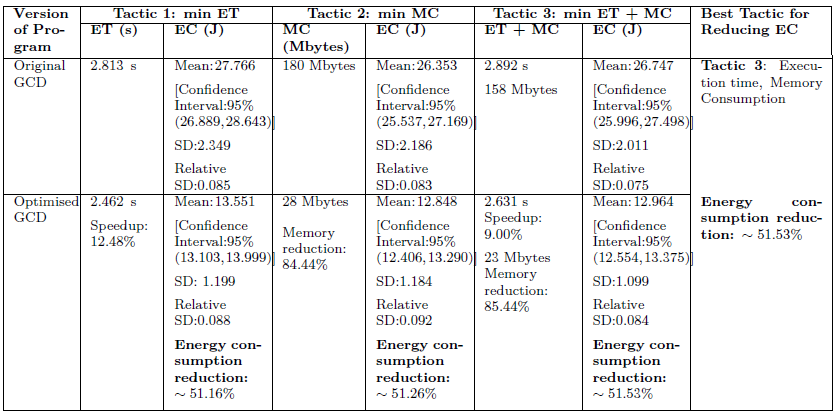
\includegraphics[width=\textwidth]{figures/Result_table_f_1.png}
    \caption*{\tiny{\textcolor{blue}{Table}: Comparison of the energy consumed by the original vs. the optimized versions of the studied programs, \textit{where: ET=execution time in seconds, MC=memory consumption in Megabytes, EC=energy consumption in Joules}}}
  \end{table}
\end{frame}

%---------- Slide 13(Research Contributions GCD)  -----------%
\begin{frame}{Main Content}
  \frametitle{Research Contributions(RQ2.1): Does the improvement of execution time and memory consumption reduce energy consumption?}

  \begin{figure}
    \centering
    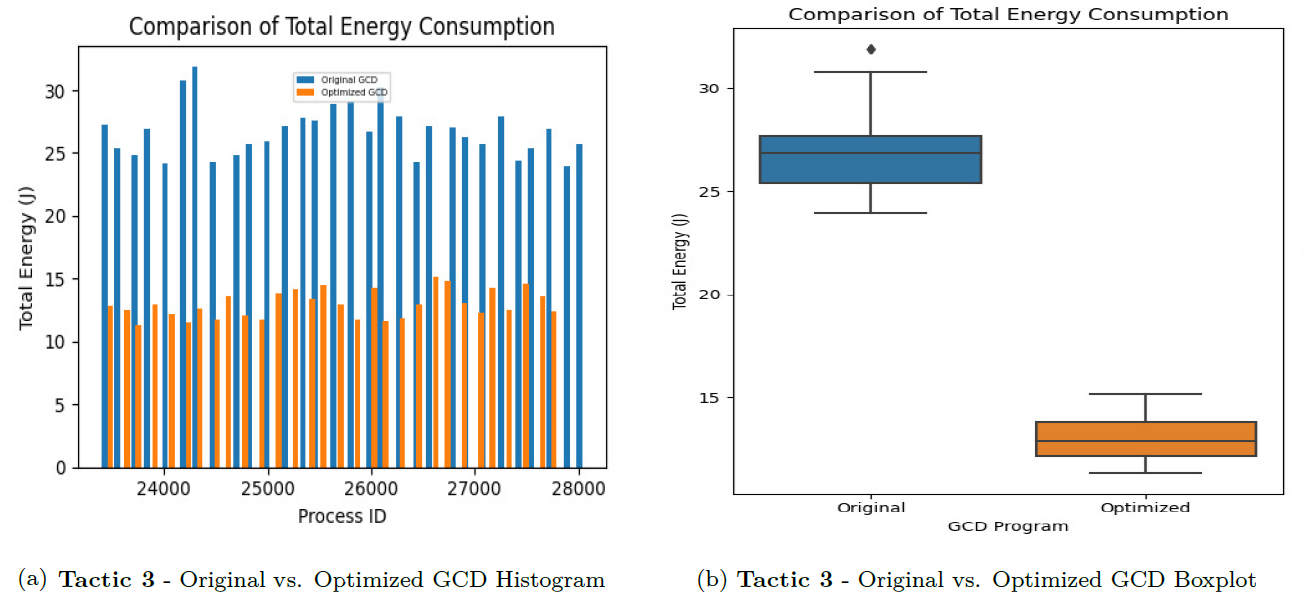
\includegraphics[width=1\textwidth]{figures/Hiegest_GCD.png}
    \caption*{\scriptsize{\textcolor{blue}{Figure}: Energy consumption comparison for the original vs. optimized versions of the \textit{Greatest Common Divisor(GCD)} program by applying the studied tactics 3}}
 \end{figure}
 
\end{frame}

%---------- Slide 14(Research Contributions)  -----------%
\begin{frame}{Main Content}
  \frametitle{Research Contributions(RQ2.1): Does the improvement of execution time and memory consumption reduce energy consumption?}
  \vspace{-.2cm}
  \begin{table}
    \centering
    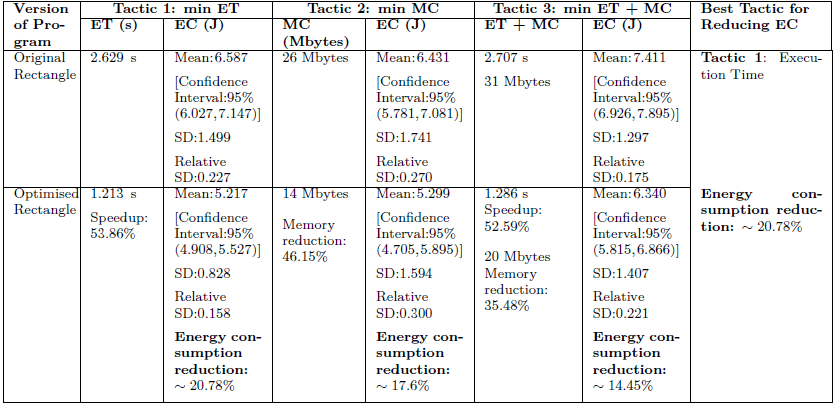
\includegraphics[width=\textwidth]{figures/Result_table_f_2.png}
    \caption*{\tiny{\textcolor{blue}{Table}: Comparison of the energy consumed by the original vs. the optimized versions of the studied programs, \textit{where: ET=execution time in seconds, MC=memory consumption in Megabytes, EC=energy consumption in Joules}}}
  \end{table}
\end{frame}

%---------- Slide 15(Research Contributions Rectangle)  -----------%
\begin{frame}{Main Content}
  \frametitle{Research Contributions(RQ2.1): Does the improvement of execution time and memory consumption reduce energy consumption?}

  \begin{figure}
    \centering
    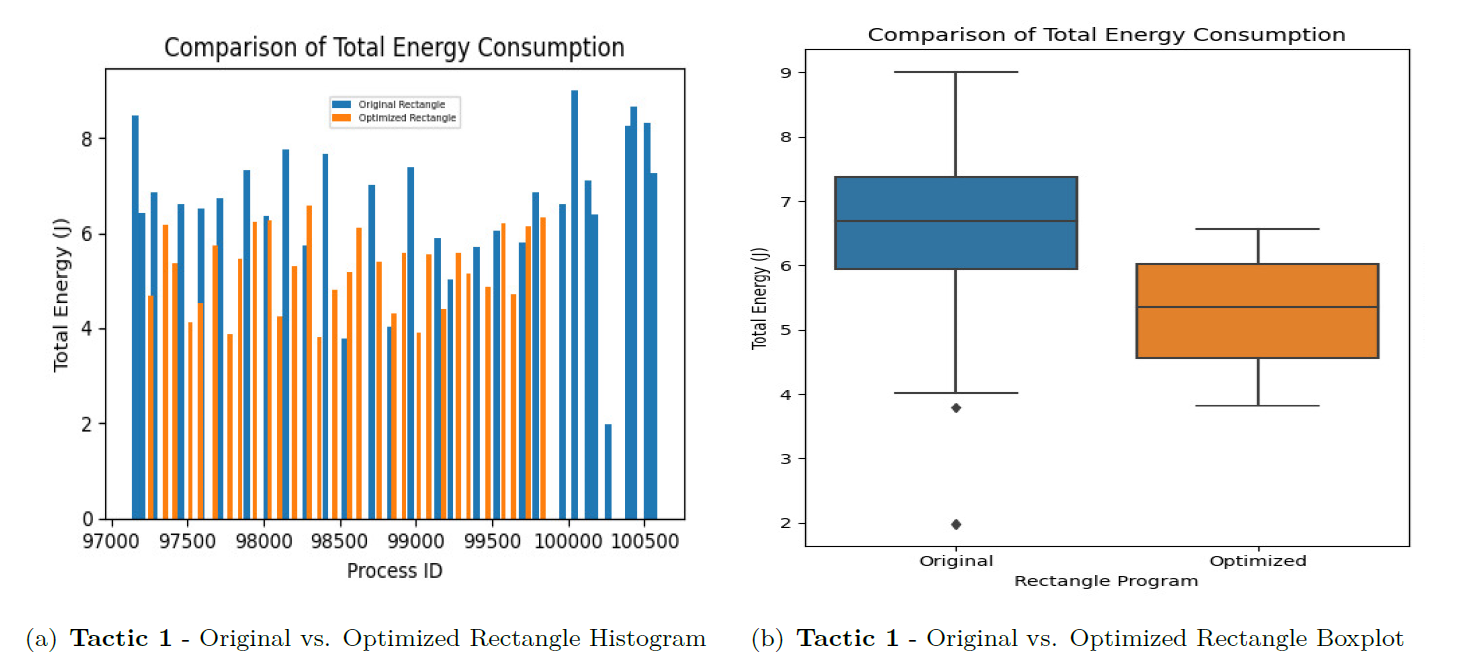
\includegraphics[width=1\textwidth]{figures/Hiegest_Rectangle.png}
    \caption*{\scriptsize{\textcolor{blue}{Figure}: Energy consumption comparison for the original vs. optimized versions of the \textit{Rectangle} program by applying the studied tactics 1}}
 \end{figure}
 
\end{frame}

%---------- Slide 16(Research Contributions)  -----------%
\begin{frame}{Main Content}
  \frametitle{Research Contributions(RQ2.2): Could code refactoring integrate into GI? Which elements need to be extended in the Gin tool?}
  
   \begin{figure}
    \centering
    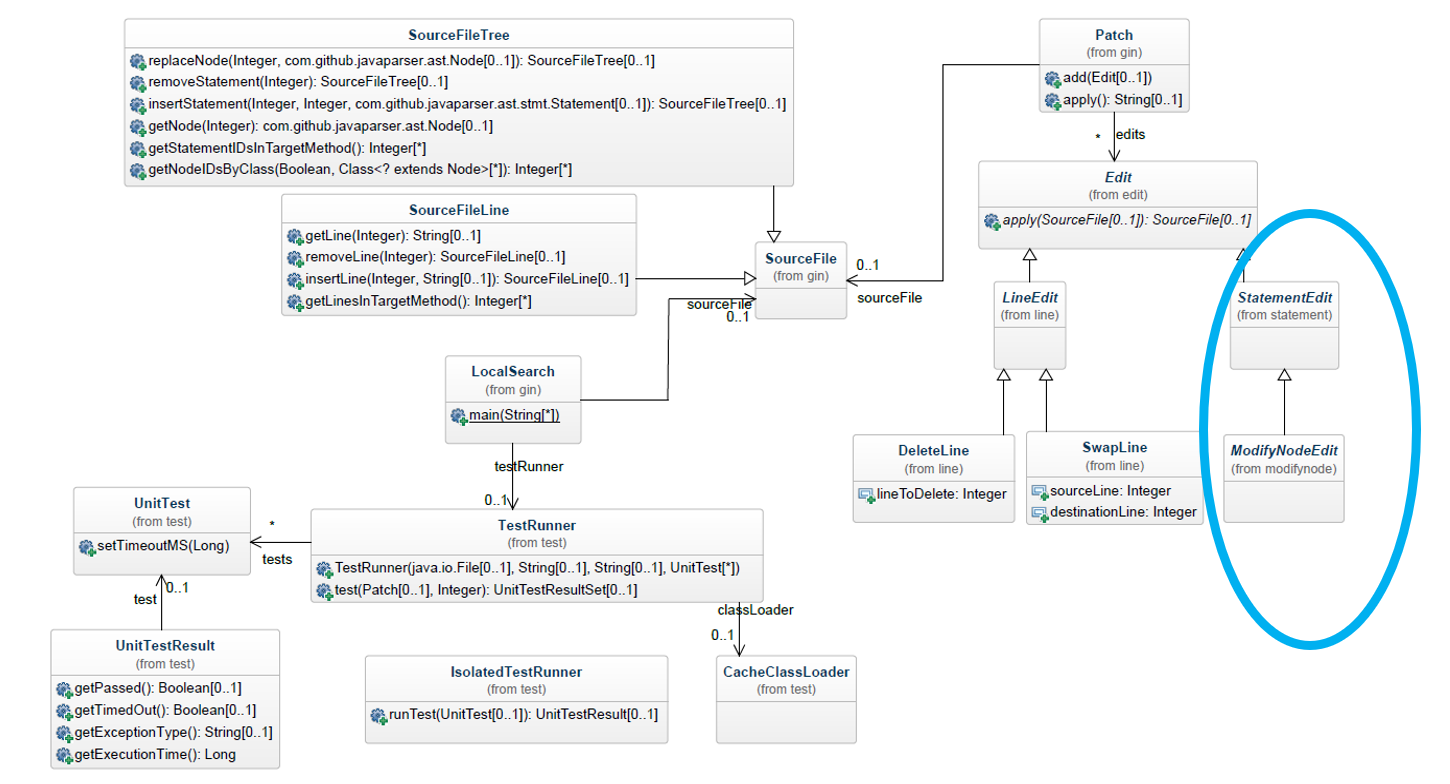
\includegraphics[width=.9\textwidth]{figures/Slide_17(Gin class diagram).png}
    \captionsetup{justification=centering} % Center the caption
    \caption*{\scriptsize{\textcolor{blue}{Figure}: Gin core classes from \cite{brownlee2019gin}}}
  \end{figure}
  
\end{frame}

%---------- Slide 17(Conclusion)  -----------%

\begin{frame}{Main Content}
 \frametitle{Conclusion}
 \vspace{-1.5cm}
 \begin{itemize}
    \item[]\footnotesize{I have Presented:}
    \begin{itemize}
        \item \footnotesize Tactics(Design Patterns, Code Refactoring,etc) for  energy-efficient software addressing \textbf{RQ1}.
        \item \footnotesize  tool for real-time energy monitoring.
        \item \footnotesize GIN tool for automation, addressing \textbf{RQ2.1} and \textbf{RQ2.2}.
    \end{itemize}
 \end{itemize}
 \vspace{1em}
\begin{itemize}
    \item[]\footnotesize{Research Contributions:}
    \begin{itemize}
        \item \footnotesize Identified code refactoring as an effective tactic(\textbf{RQ1}).
        \item \footnotesize Automated JoularJX monitoring with Bash scripts.
        \item \footnotesize Optimized programs with Gin, achieving up to 51.53\% energy reduction(\textbf{RQ2.1}).
        \item \footnotesize Identified refactoring integration opportunities in GIN's StatementEdit class(\textbf{RQ2.2}).
    \end{itemize}
\end{itemize}


 \end{frame}

%---------- Slide 18(Next Steps)  -----------%
\begin{frame}{Main Content}
  \frametitle{Next Steps}
  \vspace{-2cm}
   \textbf{\footnotesize RQ2.3}: \footnotesize In which extent code refactoring genetically improve the software to reduce energy consumption?
   
   \vspace{1em}
   \begin{enumerate}
   \item Steps for Code Smell Detection
       \begin{itemize}
        \item \footnotesize Translate Code to AST: 
        \item \footnotesize Select Detection Tool: 
        \item \footnotesize Implementation:
        \end{itemize}

   \item \footnotesize Integrate refactoring techniques post code smell detection.
   \item \footnotesize Run experiments to validate energy savings in software.
   \end{enumerate}
\end{frame}

%---------- Slide 19(References)  -----------%
\backupbegin
\begin{frame}{Main Content}
  \frametitle{References (Part 1)}
  \tiny
  \printbibliography[heading=none, keyword=part1]
\end{frame}

\begin{frame}
  \frametitle{References (Part 2)}
  \tiny
  \printbibliography[heading=none, keyword=part2]
\end{frame}

\begin{comment}
\begin{frame}
  \frametitle{References (Part 3)}
  \tiny
  \printbibliography[heading=none, keyword=part3]
\end{frame}
\end{comment}

%---------- Slide 20(Thank you)  -----------%
\begin{frame}
\frametitle{}
    \begin{figure}
    \centering
        
\includegraphics[width=1\textwidth]{figures/Slide_22(Thank_you).png}
   \end{figure}

\end{frame}
\backupend

\appendix
\section{Appendix}
%---------- Appendix -----------%
\begin{frame}
\frametitle{Appendix}
\vspace{-1.8cm}
\begin{enumerate}
    \item[]\footnotesize{\hyperlink{Intro_11}{Introduction: Why we need to reduce energy consumption in software?}}
    \item[]\footnotesize{\hyperlink{Intro_1}{Introduction: Green IT \& Green in Software Engineering}}
    \item[]\footnotesize{\hyperlink{Intro_2}{Introduction: Environmental sustainability quality attributes in software}}
    \item[]\footnotesize{\hyperlink{Research Contributions_1}{Research Contributions(RQ1): Code smells and code refactoring}}
    \item[]\footnotesize{\hyperlink{codeRefactorSlide}{Research Contributions(RQ1):Code refactoring example}}
    \item[]\footnotesize{\hyperlink{Preliminary_study}{Research Contributions: Preliminary study for empirical evaluations: Using JoularJX for Energy Monitoring in Java Program and project}}
    \item[]\footnotesize{\hyperlink{Energy_Consumption}{Research Contributions: Energy Consumption Monitoring of Java Program mandelbrot.java}}
    \item[]\footnotesize{\hyperlink{Energy_Consumption_cMath}{Research Contributions:Energy Consumption Monitoring of Project (cMath)}}
    \item[]\footnotesize{\hyperlink{Gin_toolbox}{Research Contributions(RQ2): The Gin toolbox(1/2)}}
    \item[]\footnotesize{\hyperlink{Gin_toolbox_2}{Research Contributions(RQ2): The Gin toolbox(2/2)}}
\end{enumerate}
\end{frame}

%---------- Appendix 1 (Introduction) -----------%
\begin{frame}{Main Content}
\hypertarget{Intro_11}{}
\frametitle{Introduction: Why we need to reduce energy consumption in software?}

\begin{figure}
    \vspace*{-0.4cm} % Adjust the value to change the vertical position of the pictures
    \centering
    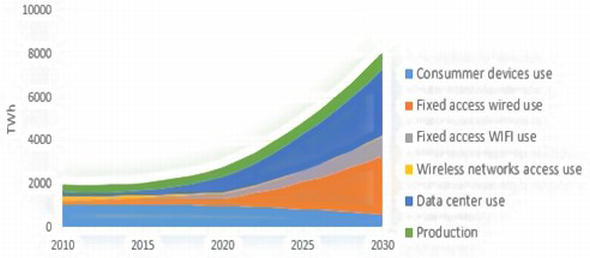
\includegraphics[width=.6\textwidth]{figures/Slide_1(ICT electricity consumption).png}
    \captionsetup{justification=centering} % Center the caption
    \caption*{\scriptsize{\textcolor{blue}{Figure}: ICT electricity consumption from \cite{muthu2019green}}}
    \label{fig:ICT electricity consumption}
 \end{figure}
 
\begin{itemize}
    \vspace*{-0.75cm} % Adjust the value to change the vertical position of the pictures
    \item \textbf{\footnotesize Direct implication:}
    \begin{itemize}
        \item \footnotesize Reduce greenhouse gas emissions and combat climate change.
        \item \footnotesize Conserve limited resources like fossil fuels and electricity generation infrastructure.
    \end{itemize}
    
    \item \textbf{\footnotesize Indirect implication:}
    \begin{itemize}
        \item \footnotesize Social Impact: Lower electricity  costs for individuals and organizations.
        \item \footnotesize Technology Impact: Promote sustainable growth and responsible technology usage.
    \end{itemize}
\end{itemize}
\end{frame}

%---------- Appendix 1 -----------%
\begin{frame}{Appendix}
\hypertarget{Intro_1}{}
  \frametitle{Green IT \& Green in Software Engineering}
  
 \begin{figure}
     \vspace*{-0.25cm} % Adjust the value to change the vertical position of the pictures
    \centering
    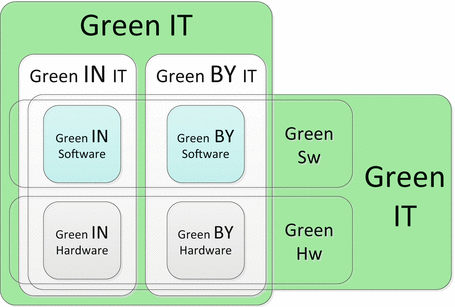
\includegraphics[width=.4\textwidth]{figures/Slide_2(Green software, green hardware and Green IT).png}
    \captionsetup{justification=centering} % Center the caption
    \caption{\small Green software, green hardware and Green IT from \cite{calero2015introduction}}
    \label{fig:Green software, green hardware and Green IT}
 \end{figure}
 
 \begin{figure}
     \vspace*{-0.5cm} % Adjust the value to change the vertical position of the pictures
    \centering
    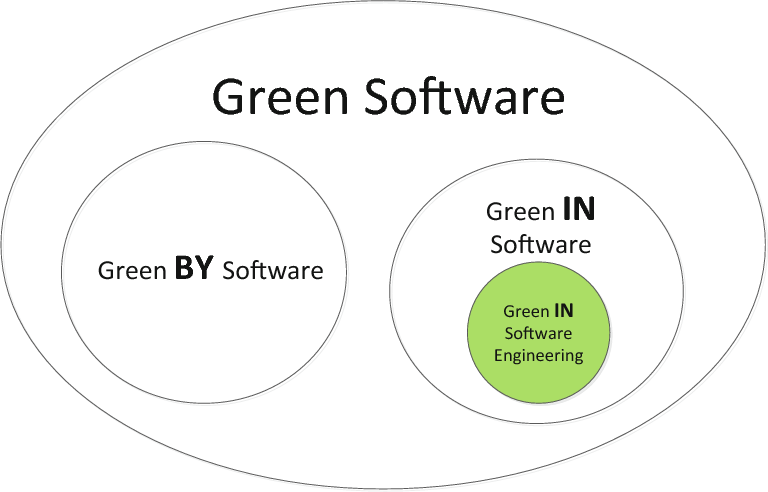
\includegraphics[width=.4\textwidth]{figures/Slide_2(Green in software engineering_1).png}
    \captionsetup{justification=centering} % Center the caption
    \caption{\small Green in software engineering from \cite{calero2015introduction}}
    \label{fig:Green software, green hardware and Green IT}
 \end{figure}
\end{frame}
%---------- Appendix 2 -----------%
\begin{frame}{Appendix}
\hypertarget{Intro_2}{}
  \frametitle{Introduction: Environmental sustainability quality attributes in software}
  \vspace*{-2cm} % Adjust the value to change the vertical position of the text
  We have two main environmental sustainability quality attributes:
    \begin{itemize}
        \item \small \textbf{Energy Awareness:} \justifying The level in which stakeholders (such developers, architects, analysts, end-users) are aware of the energy consumption involved in the building and usage of software.
        \item \small \textbf{Energy Efficiency:} \justifying The level in which a software application is able to spend less energy without affecting its functionalities. It could be at design-time or at run-time.
    \end{itemize}
\end{frame}
%---------- Appendix 3 -----------%
\begin{frame}{Appendix}
\hypertarget{Research Contributions_1}{}
  \frametitle{Research Contributions(RQ1): Code smells and code refactoring (1/2)}
\vspace{-.4cm}
%\scriptsize
\tiny
\begin{table}[!t]
\centering
\caption{Comparison of approaches}\label{tab:result}
\vspace{-.4cm}
%\centering
\begin{tabular}{|p{1.5cm}|p{3cm}|p{2.5cm}|p{2cm}|p{1cm}|}

\hline
\textbf{Reference} & \textbf{Code refactoring} & \textbf{Experiment / Bench-marking} & \textbf{Tool for EC} & \textbf{Results}  \\

\hline
\cite{sahin2014code} & 
\textbf{Code Refactoring(6)}:\textcolor{darkgreen}{Convert Local Variable to Field},
Extract Local Variable,
Extract Method,
Introduce Indirection, 
Inline Method,
\textcolor{darkgreen}{Introduce Parameter Object} & 
9 Java Applications (ex. cMath, cCollections, ..) & 
Low Power Energy Aware Process (LEAP) & 
-7.50\% to 4.54\%  \\
\hline

\cite{morales2018earmo} & 
\textbf{Android code smells (3)}: Binding resources too early class, Private getter and setters, HashMap usage. \textbf{OO code smells (5)}: Lazy class, Blob (God class), Long-parameter list, Refused bequest, Speculative Generality & 
\textbf{Phase 1:} Empirical Study to understand in which extent 8 code refactorings help to save energy. 
\textbf{Phase 2:} EARMO is developped to select optimal series of code refactoring.  The energy consumed by the version of code is inferred from Phase 1. & 
Not reported. &
Removes a median of 84\% of code smells or anti-patterns,able to save 29 minutes of battery.
\\
\hline

\cite{palomba2019impact} & 
\textbf{Android-specific code smells (9)}: Data Transmission Without Compression, Durable Wakelock, Inefficient Data Structure, Inefficient SQL Query, Inefficient Data Format And Parser, \textcolor{red}{Internal Setter, Leaking Thread,  Member-Ignoring Method, Slow Loop} & 
60 Android Java apps (categories ex. games, productivity, social, etc) & 
PETRA (Power Estimation Tool for Android) & 
Four code smell types increase method energy consumption by up to 87 times.
\\
\hline

\end{tabular}
\end{table}

\end{frame}

%---------- Appendix 4 -----------%
\begin{frame}{Appendix}
\hypertarget{codeRefactorSlide}{}
  \frametitle{Research Contributions(RQ1):\hyperlink{back} {Code refactoring example} }
  \begin{figure}[t]
    \begin{minipage}[t]{0.45\textwidth}
        \raggedleft
        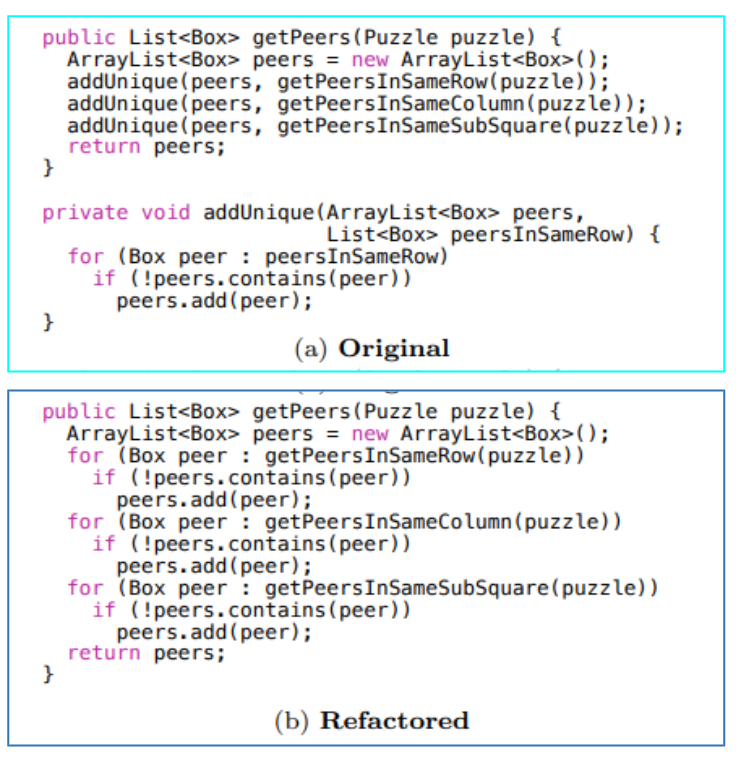
\includegraphics[width=\textwidth]{figures/Slide_13_2(Inline code refactoring example).png}
        \captionsetup{singlelinecheck=false, justification=centering}
        \caption{\small Inline method code refactoring example from \cite{sahin2014code}}
        \label{fig:Inline code refactoring example}
    \end{minipage}
\end{figure}

\end{frame}

%---------- Appendix 5 -----------%
\begin{frame}{Appendix}
\label{appendix}
\hypertarget{Preliminary_study}{}
\frametitle{Research Contributions: Preliminary study for empirical evaluations: Using JoularJX for Energy Monitoring in Java Program and project}

\begin{itemize}
    \item \textbf{Tool Used:} JoularJX
    \begin{itemize}
        \item Monitors energy consumption at the Java method level.
    \end{itemize}
    
    \item \textbf{Installation Guidelines:}
    \begin{itemize}
        \item Followed from \href{https://github.com/joular/joularjx}{JoularJX GitHub Repository}.
    \end{itemize}
    
    \item \textbf{Minimum Requirements:}
    \begin{itemize}
        \item Java 11+
    \end{itemize}
    
    \item \textbf{Platform Dependencies:}
    \begin{itemize}
        \item Windows: Intel Power Gadget API
        \item GNU/Linux: Intel RAPL through powercap
    \end{itemize}
    
    \item \textbf{Test Environment:}
    \begin{itemize}
        \item Dell Latitude 7490 with Intel Core i7-8650U CPU
        \item Running Debian GNU/Linux 11 (bullseye) \& Java 17
    \end{itemize}
\end{itemize}

\end{frame}

%---------- Appendix 6 -----------%


\begin{frame}{Appendix}
\label{appendix}
\hypertarget{Energy_Consumption}{}
  \frametitle{Research Contributions: Energy Consumption Monitoring of Java Program (\href{https://en.wikipedia.org/wiki/Mandelbrot_set}{mandelbrot.java})}
  
  \begin{figure}
     \vspace*{-.5cm} % Adjust the value to change the vertical position of the pictures
    \centering
    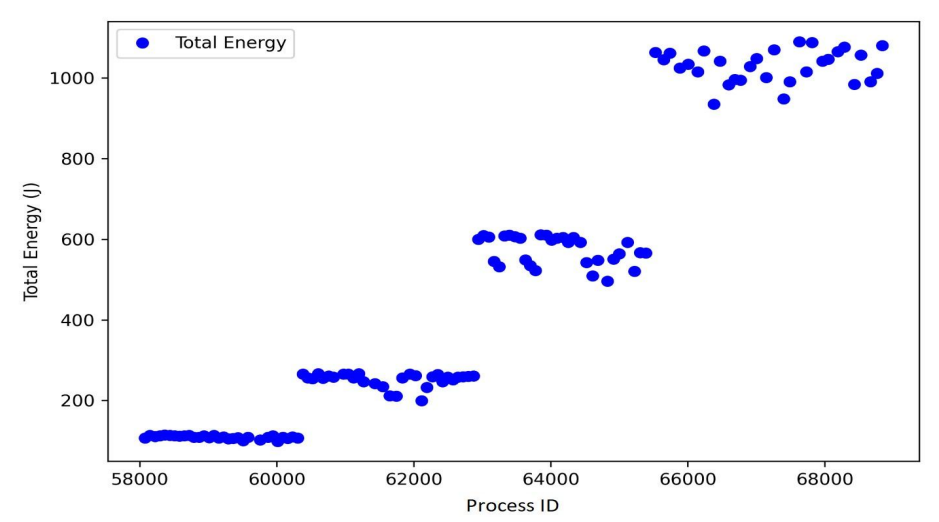
\includegraphics[width=.7\textwidth]{figures/Slide_8(Total energy consumption for each Process ID).png}
    \captionsetup{justification=centering} % Center the caption
    \caption{\small Total energy consumption for each Process ID }
    \label{fig:Total energy consumption for each Process ID}
 \end{figure}
 
 \begin{picture}(0,0)
   \put(250,8){
\includegraphics[height=.5cm]{figures/Slide_8_9(joularjx_logo).png}}
   \put(240,2){\href{https://github.com/joular/joularjx}{\textcolor{gray}{\tiny https://github.com/joular/joularjx}}}
 \end{picture}

\end{frame}

%---------- Appendix 7 -----------%

\begin{frame}{Appendix}
\label{appendix}
\hypertarget{Energy_Consumption_cMath}{}
  \frametitle{Research Contributions: Energy Consumption Monitoring of Project (cMath)}
  
  \vspace*{-.8cm} % Adjust the value to change the vertical position of the pictures
  
  \begin{figure}[t]
    \begin{minipage}[t]{0.55\textwidth}
        \raggedright
        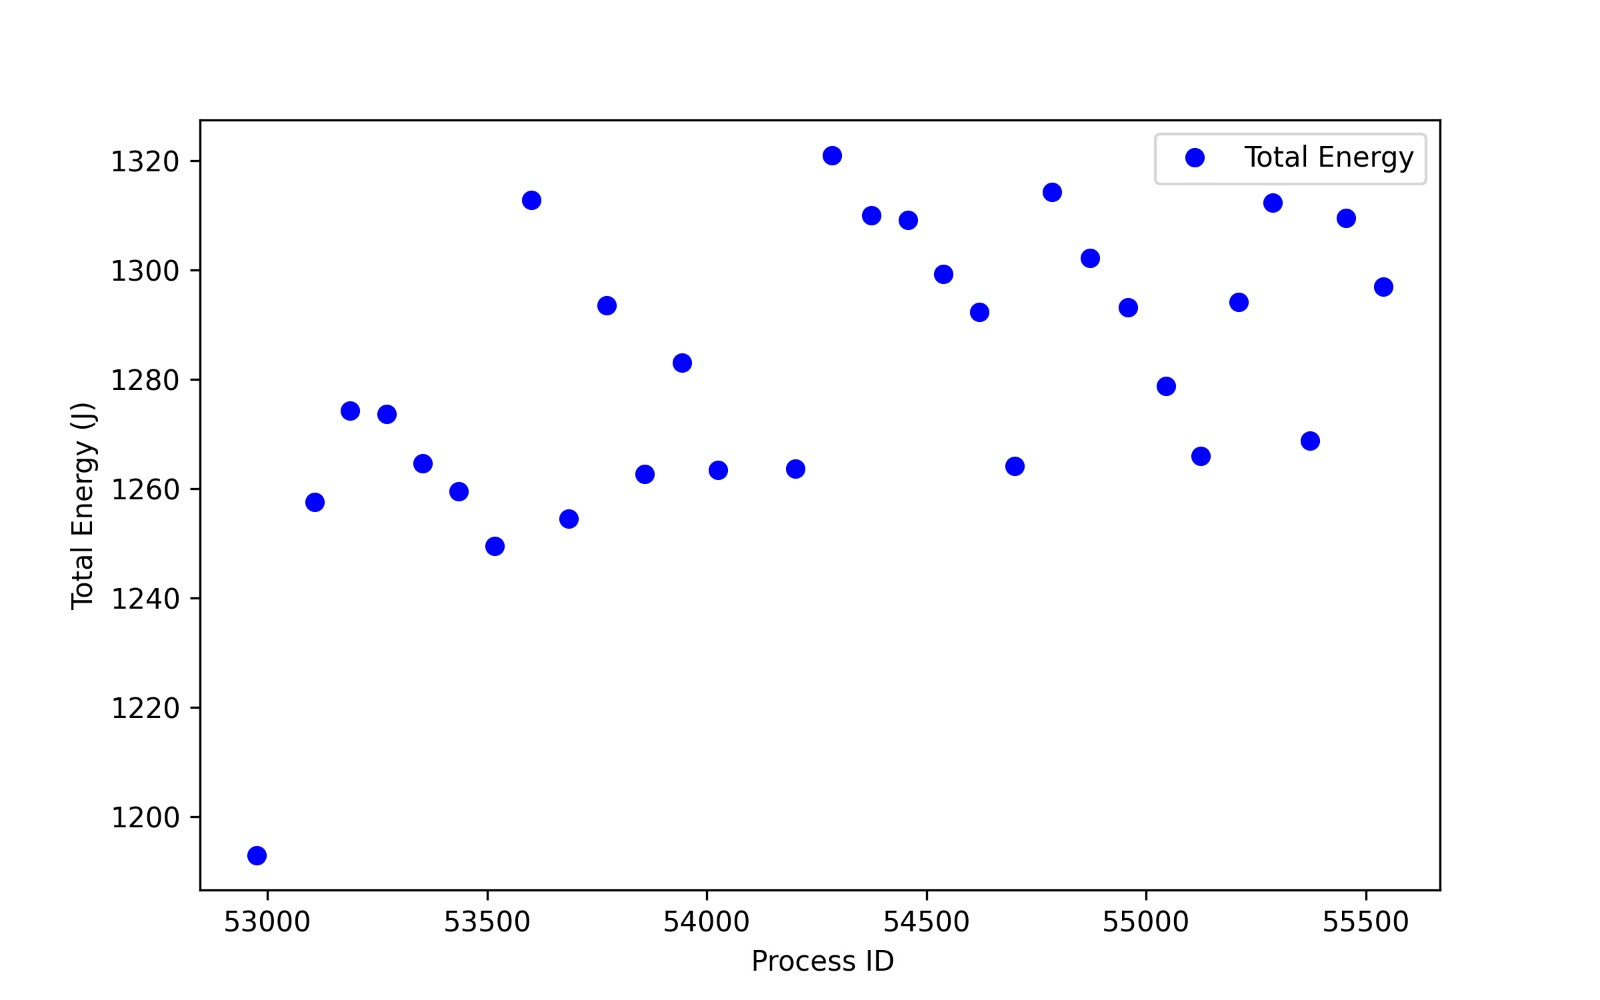
\includegraphics[width=\textwidth]{figures/cMath_project_energy.jpeg}
        \captionsetup{singlelinecheck=false, justification=centering}
        \caption{\small Total energy consumption for each Process ID}
        \label{fig:Total energy consumption for each Process ID}
    \end{minipage}\hfill
    \begin{minipage}[t]{0.45\textwidth}
        \raggedleft
        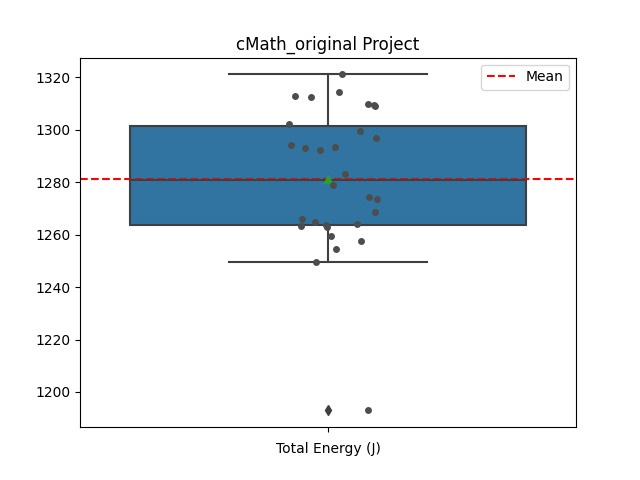
\includegraphics[width=\textwidth]{figures/cMath_project_energy_boxplot.jpeg}
        \captionsetup{singlelinecheck=false, justification=centering}
        \captionsetup{justification=centering} % Center the caption
        \caption{\small Boxplot of  total energy consumption for each Process ID}
        \label{fig:Boxplot of  total energy consumption for each Process ID}
    \end{minipage}
\end{figure}

 \begin{picture}(0,0)
   \put(250,-13){
\includegraphics[height=.5cm]{figures/Slide_8_9(joularjx_logo).png}}
   \put(240,-19){\href{https://github.com/joular/joularjx}{\textcolor{gray}{\tiny https://github.com/joular/joularjx}}}
 \end{picture}
 
 
 
\end{frame}

%---------- Slide 8 -----------%


\begin{frame}{Appendix}
\label{appendix}
\hypertarget{Gin_toolbox}{}
  \frametitle{Research Contributions(RQ2): The Gin toolbox(1/2)}
  
   \begin{figure}
    \centering
    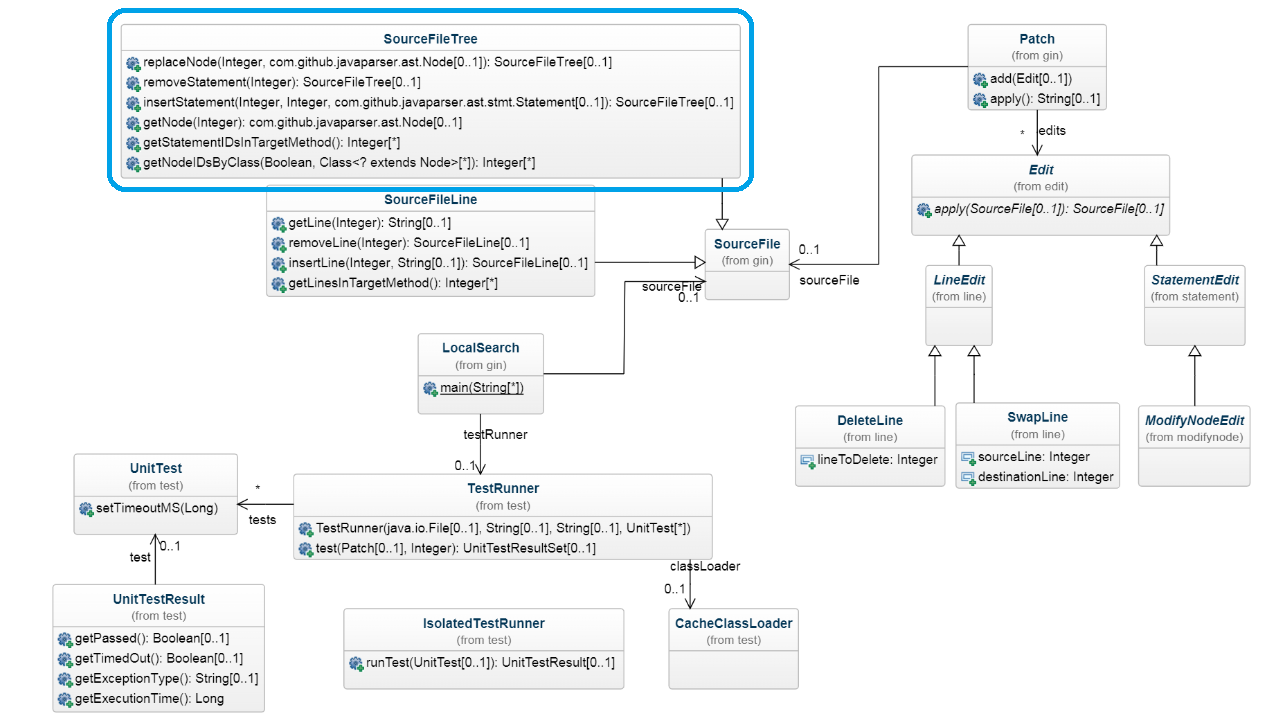
\includegraphics[width=1\textwidth]{figures/Slide_18(Gin class diagram).png}
    \captionsetup{justification=centering} % Center the caption
    \caption{Gin core classes from \cite{brownlee2019gin}}
  \end{figure}
  
\end{frame}

%---------- Slide 9 -----------%
\begin{frame}{Appendix}
\label{appendix}
\hypertarget{Gin_toolbox_2}{}
  \frametitle{Research Contributions(RQ2): The Gin toolbox(2/2)}
  
   \begin{figure}
    \centering
    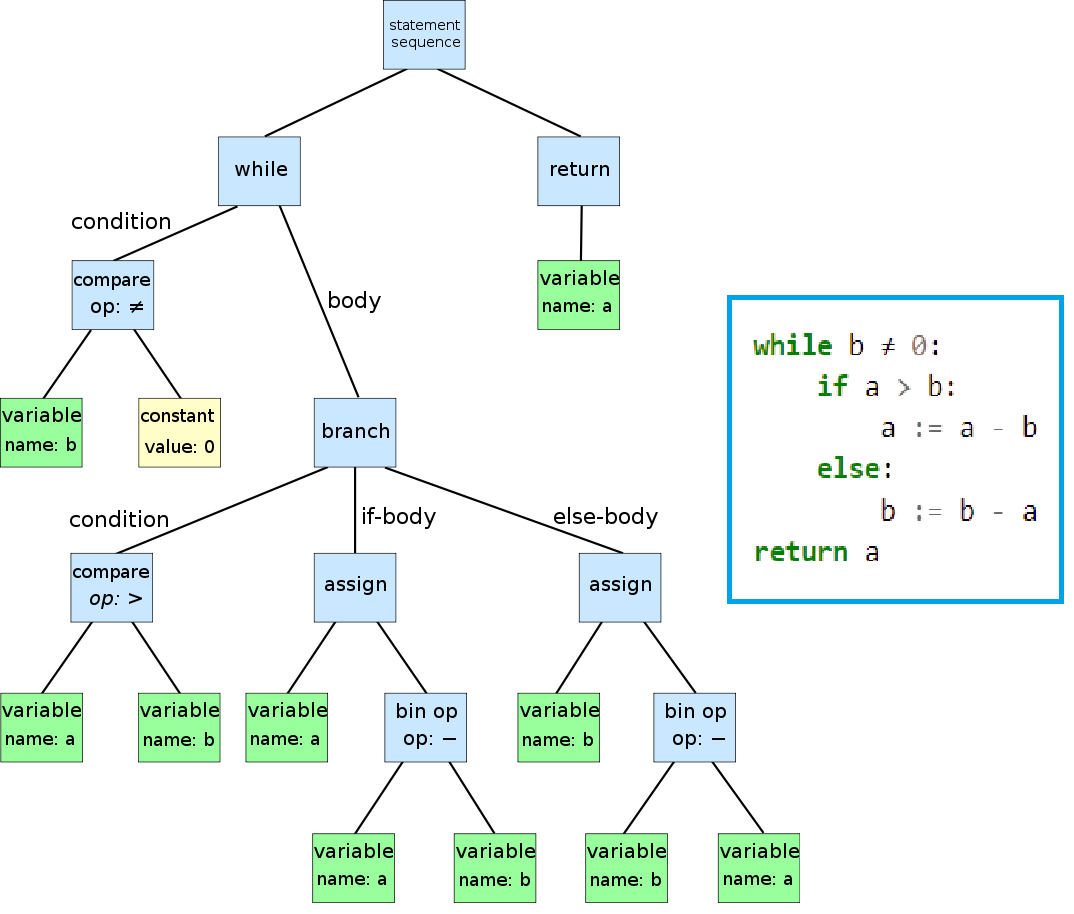
\includegraphics[width=.7\textwidth]{figures/Slide_19(Abstract syntax tree).png}
    \captionsetup{justification=centering} % Center the caption
    \caption{Abstract Syntax Tree from \cite{hung2014rule}}
  \end{figure}
  
\end{frame}



\end{document}

